%%%%%%%%%%%%%%%%%%%%%%%%%%%%%%%%%%%%%%%%%%%%%%%%%%%%%%%%%%%%%%%%%%%%%%%%%%%
%% This file is part of the book
%%
%% Algorithmic Graph Theory
%% http://code.google.com/p/graph-theory-algorithms-book/
%%
%% Copyright (C) 2009, 2010, 2011 Minh Van Nguyen <nguyenminh2@gmail.com>
%%
%% See the file COPYING for copying conditions.
%%%%%%%%%%%%%%%%%%%%%%%%%%%%%%%%%%%%%%%%%%%%%%%%%%%%%%%%%%%%%%%%%%%%%%%%%%%

\documentclass{article}

\usepackage{subfigure}
\usepackage{tikz}
\usetikzlibrary{external}
\tikzexternalize{various-r-regular-graphs}

\begin{document}

\begin{figure}
\subfigure[]{
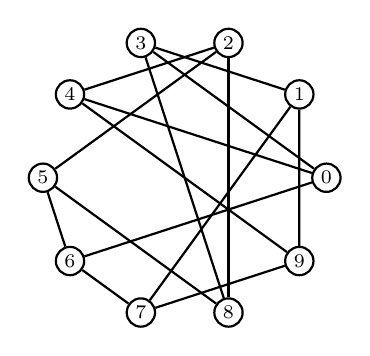
\begin{tikzpicture}
[lineDecorate/.style={-,thick},%
  nodeDecorate/.style={shape=circle,inner sep=1.5pt,draw,thick},
  scale=1.8]
\scriptsize
%% nodes or vertices
\foreach \nodename/\x/\y in {
  0/1.00000000000000/0.000000000000000,
  1/0.809016994374947/0.587785252292473,
  2/0.309016994374947/0.951056516295154,
  3/-0.309016994374947/0.951056516295154,
  4/-0.809016994374947/0.587785252292473,
  5/-1.00000000000000/0.000000000000000,
  6/-0.809016994374947/-0.587785252292473,
  7/-0.309016994374947/-0.951056516295154,
  8/0.309016994374947/-0.951056516295154,
  9/0.809016994374947/-0.587785252292473}
{
  \node (\nodename) at (\x,\y) [nodeDecorate] {$\nodename$};
}
%% edges or lines
\path
\foreach \startnode/\endnode in {
  0/3, 0/4, 0/6, 1/3, 1/7, 1/9, 2/4, 2/5, 2/8, 3/8, 4/9, 5/6, 5/8,
  6/7, 7/9}
{
  (\startnode) edge[lineDecorate] node {} (\endnode)
};
\end{tikzpicture}
}
%%
%%
\qquad
\subfigure[]{
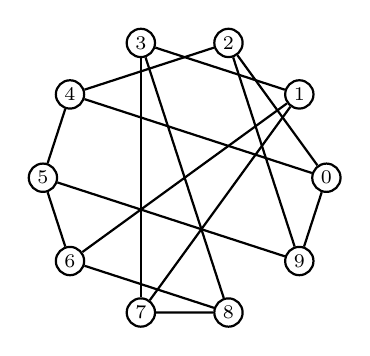
\begin{tikzpicture}
[lineDecorate/.style={-,thick},%
  nodeDecorate/.style={shape=circle,inner sep=1.5pt,draw,thick},
  scale=1.8]
\scriptsize
%% nodes or vertices
\foreach \nodename/\x/\y in {
  0/1.00000000000000/0.000000000000000,
  1/0.809016994374947/0.587785252292473,
  2/0.309016994374947/0.951056516295154,
  3/-0.309016994374947/0.951056516295154,
  4/-0.809016994374947/0.587785252292473,
  5/-1.00000000000000/0.000000000000000,
  6/-0.809016994374947/-0.587785252292473,
  7/-0.309016994374947/-0.951056516295154,
  8/0.309016994374947/-0.951056516295154,
  9/0.809016994374947/-0.587785252292473}
{
  \node (\nodename) at (\x,\y) [nodeDecorate] {$\nodename$};
}
%% edges or lines
\path
\foreach \startnode/\endnode in {
  0/2, 0/4, 0/9, 1/3, 1/6, 1/7, 2/4, 2/9, 3/7, 3/8, 4/5, 5/6, 5/9,
  6/8, 7/8}
{
  (\startnode) edge[lineDecorate] node {} (\endnode)
};
\end{tikzpicture}
}
%%
%%
\qquad
\subfigure[]{
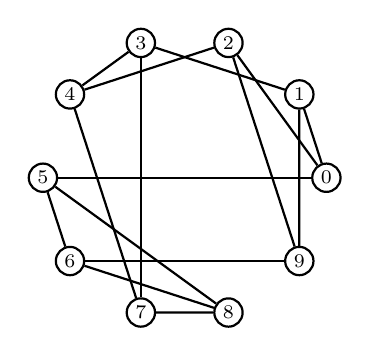
\begin{tikzpicture}
[lineDecorate/.style={-,thick},%
  nodeDecorate/.style={shape=circle,inner sep=1.5pt,draw,thick},
  scale=1.8]
\scriptsize
%% nodes or vertices
\foreach \nodename/\x/\y in {
  0/1.00000000000000/0.000000000000000,
  1/0.809016994374947/0.587785252292473,
  2/0.309016994374947/0.951056516295154,
  3/-0.309016994374947/0.951056516295154,
  4/-0.809016994374947/0.587785252292473,
  5/-1.00000000000000/0.000000000000000,
  6/-0.809016994374947/-0.587785252292473,
  7/-0.309016994374947/-0.951056516295154,
  8/0.309016994374947/-0.951056516295154,
  9/0.809016994374947/-0.587785252292473}
{
  \node (\nodename) at (\x,\y) [nodeDecorate] {$\nodename$};
}
%% edges or lines
\path
\foreach \startnode/\endnode in {
  0/1, 0/2, 0/5, 1/3, 1/9, 2/4, 2/9, 3/4, 3/7, 4/7, 5/6, 5/8, 6/8,
  6/9, 7/8}
{
  (\startnode) edge[lineDecorate] node {} (\endnode)
};
\end{tikzpicture}
}
\end{figure}

\end{document}
